\section{Εργαλεία Λογισμικού}
\label{sec:dnn_sw}

Εξαιτίας της ραγδαίας εξέλιξης της επιστήμης της βαθιάς μηχανικής μάθησης,
τα τελευταία χρόνια έχουν αναπτυχθεί πολλά εργαλεία λογισμικού (βιβλιοθήκες, SDKs, frameworks)
για γρήγορη ή/και αποτελεσματική σχεδίαση και υλοποίηση πολυεπίπεδων νευρωνικών δικτύων.

Μερικά από τα πιο γνωστά εργαλεία
σχεδίασης και ανάπτυξης αλγορίθμων και μοντέλων πολυεπίπεδων νευρωνικών δικτύων, τα οποία
χρησιμοποιούνται από την επιστημονική κοινότητα είναι:
\begin{itemize}
  \item{Caffe \footnote{\url{http://caffe.berkeleyvision.org/}} %
      \cite{jia2014caffe}:
    Framework για σχεδίαση, υλοποίηση και δοκιμή μοντέλων βαθιάς μηχανικής μάθησης.
    Είναι ένα από τα πρώτα ανοικτού κώδικα εργαλεία βαθιάς μηχανικής μάθησης που αναπτύχθηκαν.}
  \item{Tensorflow \footnote{\url{https://www.tensorflow.org/}} %
      \cite{DBLP:journals/corr/AbadiBCCDDDGIIK16}:
    Ανοικτού κώδικα βιβλιοθήκη για αριθμητικούς υπολογισμούς χρησιμοποιώντας
    γράφους ροής δεδομένων ανεπτυγμένο από την ερευνητική ομάδα της Google.
    Η ευέλικτη αρχιτεκτονική της επιτρέπει την ανάπτυξη
    λογισμικού σε μία ή και περισσότερες κεντρικές μονάδες επεξεργασίας CPU ή μονάδες GPU.}
  \item{Theano \footnote{\url{http://deeplearning.net/software/theano/}}
      \cite{2016arXiv160502688full}\cite{bergstra+al:2010-scipy}\cite{Bastien-Theano-2012}: %
      Βιβλιοθήκη για Python η οποία επιτρέπει τον ορισμό, βελτιστοποίηση και αξιολόγηση
      μαθηματικών συναρτήσεων που αφορούν πράξεις με πολυδιάστατους πίνακες.}
  \item{Torch \footnote{\url{http://torch.ch/}} %
      \cite{collobert2002torch}\cite{collobert2011torch7}\cite{collobert2012implementing}:
    Framework για γρήγορη ανάπτυξη και δοκιμή αλγορίθμων μηχανικής μάθησης.}
  \item{Keras \footnote{\url{https://keras.io/}} \cite{chollet2015keras}:
      Ανοικτού κώδικα, υψηλού επιπέδου βιβλιοθήκη σε Python για σχεδίαση και ανάπτυξη
      πολυεπίπεδων νευρωνικών δικτύων. Ενσωματώνει
      τις βιβλιοθήκες Theano και Tensorflow.} %WTF
  \item{CNTK\footnote{\url{https://www.cntk.ai/}} \cite{Seide:2016:CMO:2939672.2945397}:
    Σετ από εργαλεία για εφαρμογές βαθιάς μηχανικής μάθησης, ανεπτυγμένο από την ερευνητική ομάδα της Microsoft.}
\end{itemize}

Όλα τα προαναφερθέντα εργαλεία χρησιμοποιούν μοντέλα γράφων
για την συμβολική αναπαράσταση των μαθηματικών υπολογισμών. Η αναπαράσταση σε μορφή γράφων
έχει αποδειχθεί αποτελεσματική όσον αφορά την ταχύτητα υπολογισμών μαθηματικών εκφράσεων, αλλά και την
απλότητα ανάπτυξης \autoref{fig:graph_model_example}.

\begin{figure}[!ht]
  \centering
  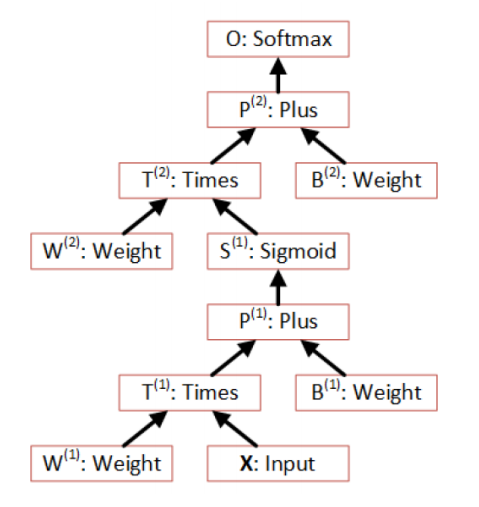
\includegraphics[width=0.6\textwidth]{./images/chapter4/graph_model_example.png}
  \caption[Παράδειγμα αναπαράστασης ενός μοντέλου νευρωνικού δικτύου σε γράφο.
    Το ΝΝ αποτλείται από ένα κρυφό επίπεδο
    και ένα ταξινομητή Sotfmax στο επίπεδο εξόδου]{
    Παράδειγμα αναπαράστασης ενός μοντέλου νευρωνικού δικτύου σε γράφο.
    Το ΝΝ απειλείται από ένα κρυφό επίπεδο με συνάρτηση ενεργοποίησης την σιγμοειδή συνάρτηση
    και έναν ταξινομητή Sotfmax στο επίπεδο εξόδου}
  \label{fig:graph_model_example}
\end{figure}
Οι κόμβοι στον γράφο αναπαριστούν μαθηματικές πράξεις ή εκφράσεις, ενώ τα φύλλα
αναπαριστούν πολυδιάστατους πίνακες δεδομένων, οι οποίοι ονομάζονται Tensors.

Η αναπαράσταση των νευρωνικών δικτύων σε μορφή γράφου ροής
δεδομένων προσθέτει ένα επίπεδο ευελιξίας στην ανάπτυξη τους. Μία σημαντική παρατήρηση
είναι ότι ο γράφος μπορεί χωριστεί σε μικρότερους υπογράφους και άρα να κατανεμηθεί
σε περισσότερες από μία υπολογιστικές μονάδες (CPUs / GPUs) ή ακόμα και
σε ετερογενή κατανεμημένα συστήματα (CPUs + GPUs) \cite{DBLP:journals/corr/AbadiABBCCCDDDG16} .

Ένα ακόμη αξιοσημείωτο εργαλείο είναι η βιβλιοθήκη \emph{ConvNetJS} \cite{karpathy2014convnetjs},
η οποία αναπτύχθηκε από τον Andrej Karpathy και υποστηρίζεται απευθείας από σύγχρονους
Web Browsers
\footnote{Στον ιστοχώρο \url{http://cs.stanford.edu/people/karpathy/convnetjs/}
υπάρχουν παραδείγματα μοντέλων νευρωνικών δικτύων τα οποία μπορεί ο αναγνώστης να δοκιμάσει
κατευθείαν μέσα από τον browser του}
ή/και σε υπολογιστικά συστήματα
\footnote{Η βιβλιοθήκη ConvNetJS μπορεί να τρέξει σε συστήματα τα οποία
υποστηρίζουν Node.js (server-side javascript interpreter)}.

Στα πλαίσια της παρούσας διπλωματικής εργασίας επιλέχθηκε να χρησιμοποιηθεί
η βιβλιοθήκη \emph{Keras} για τους εξής λόγους:
\begin{itemize}
  \item{Προσφέρει υψηλού επιπέδου ρουτίνες για ανάπτυξη νευρωνικών δικτύων}
  \item{Εύκολη και γρήγορη σχεδίαση και ανάπτυξη}
  \item{Υποστηρίζει Νευρωνικά Δίκτυα Συνέλιξης}
  \item{Παρέχει πολλά παραδείγματα σχεδίασης και ανάπτυξης}
  \item{Τρέχει σε CPU και GPU}
  \item{Επιτρέπει την επιλογή μεταξύ των βιβλιοθηκών Theano και Tensorflow
    για την εκτέλεση των μαθηματικών εκφράσεων}
  \item{Είναι από τα πιο ενεργά προγράμματα ανάπτυξης λογισμικού για DL}
\end{itemize}

Το τελευταίο σημείο είναι σημαντικό, αφού επιτρέπει την ανάπτυξη μοντέλων και
την αξιολόγηση της απόδοσή τους, κυρίως σε χρόνο εκτέλεσης,
με χρήση τόσο του Theano αλλά και του Tensorflow, χωρίς να χρειαστεί
επαναπρογραμματισμός.

Η πλήρης λίστα των εργαλείων λογισμικού που χρησιμοποιήθηκαν παρουσιάζεται πιο κάτω:
\begin{itemize}
  \item{Γλωσσα προγραμματισμού Python}
  \item{Keras: Σχεδίαση και ανάπτυξη των CNN}
  \item{Theano: Keras backend που χρησιμοποιείται για τους υπολογισμούς των μαθηματικών εκφράσεων}
  \item{Matplotlib\footnote{\url{http://matplotlib.org/}}: Βιβλιοθήκη Python για κατασκευή διαγραμμάτων}
  \item{PyDot\footnote{\url{https://pypi.python.org/pypi/pydot}}: Βιβλιοθήκη Python για κατασκευή γράφων}
\end{itemize}
